%%% Ende
\chapter{Komponentendiagramm}
Das Komponentendiagramm, \ref{pic:Softwarekompo}, dient als Anschauungsbeispiel für die Möglichkeiten der Konfiguration des Metamodels.
\section{Ports}
Zwischen den einzelnen Softwarekomponenten ist nur eine Verbindung mit Sender/Reciever Ports und Trigger Ports möglich. Auf die Basissoftware können Softwarekomponenten nur mit Server/Client Ports verbunden werden.
\section{Runnables}
Den Softwarekomponenten können Runnables zugewiesen werden, die die Ports der jeweiligen Softwarekomponente benutzen, was auch aus dem angefügten Komponentendiagramm gut ersichtlich ist.
\section{Darstellung des Komponentendiagramm}
Aus dem Komponentendiagramm, ist die Struktur unseres Projektes dargestellt. Die Darstellung umfasst dabei die verwendeten Komponenten mit deren Interfaces bzw Ports. Darüber hinaus zeigt es seine Abhängigkeitsbeziehungen und Verbindungen der Komponenten untereinander. Um das Innere einer Komponente besser zu verstehen wurden hier nochmal seine Runnable Entities aufgeführt. Der Aufbau besteht aus 4 Software Komponenten wobei SWC1, SWC3 und SWC4 aus Sensor-Aktor-Software-Komponente bestehen und lediglich SWC2 eine Anwendungssoftwarekomponente ist.

\subsection{Aufbau der ersten Software Komponente}
Die erste Software Komponente(im Diagramm als SWC1 gekennzeichnet) besitzt 3 Runnable Entities:
\begin{enumerate}
\item Joystick auslesen
\item Ultraschall auslesen
\item Flankenerkennung (auch genannt Flankensteuerung)
\end{enumerate}
Die Aufgabe dieser Softwarekomponente ist das Empfangen der Werte aus dem ADC, I$^2$C und DIO über ihre Interfaces, sowie die Weiterleitung der Werte aus den 3 Runnable Entities an die SWC2 und SWC4.

\subsection{Zweite Software Komponente}
Die Zweite Software Kompontente besteht lediglich aus der Runnable Entität \dq Werte berechnen\dq, wessen Aufgabe es ist, Werte aus der Drehzahlsteuerung aus SWC3 zu empfangen und mit den Werten des Joysticks von SWC1 zu verrechnen und wieder an die Motorsteuerung in SWC3 zu schicken.

\subsection{Dritte Software Komponente}
Bestehend aus 3 Runnable Entities hat die dritte Software Komponente (im Diagramm als SWC3 gekennzeichnet):
\begin{enumerate}
\item Motorsteuerung
\item Blinksteuerung
\item Drehzahlsteuerung
\end{enumerate}
Zu den Aufgabe der dritte Software Komponente gehört es den Motor anzusteuern und dessen Drehzahl auszulesen, sowie diese Drehzahlwerte weiter an die Softwarekomponte Zwei(SWC2) zu senden. Zudem gehört es zu seinen Aufgaben ein Blinklichtmuster an das DIO weiter zu leiten.

\subsection{Vierte Software Komponente}
Bei der vierten Software Komponente (im Diagramm als SWC4 gekennzeichnet) gibt es 2 Runnable Entities:
\begin{enumerate}
\item Display-Ausgabe
\item Sound-Ausgabe
\end{enumerate}
Zu den Aufgaben der vierten Software Komponente gehört es den Sound, sowie die Displayausgabe anzusteuern. Die Soundausgabe erfolgt über den Joystick, während das Display die Ultraschallwerte aus SWC1 entgegen nimmt und ausgibt.
\clearpage
\newpage
\begin{landscape}
\begin{figure}[h]
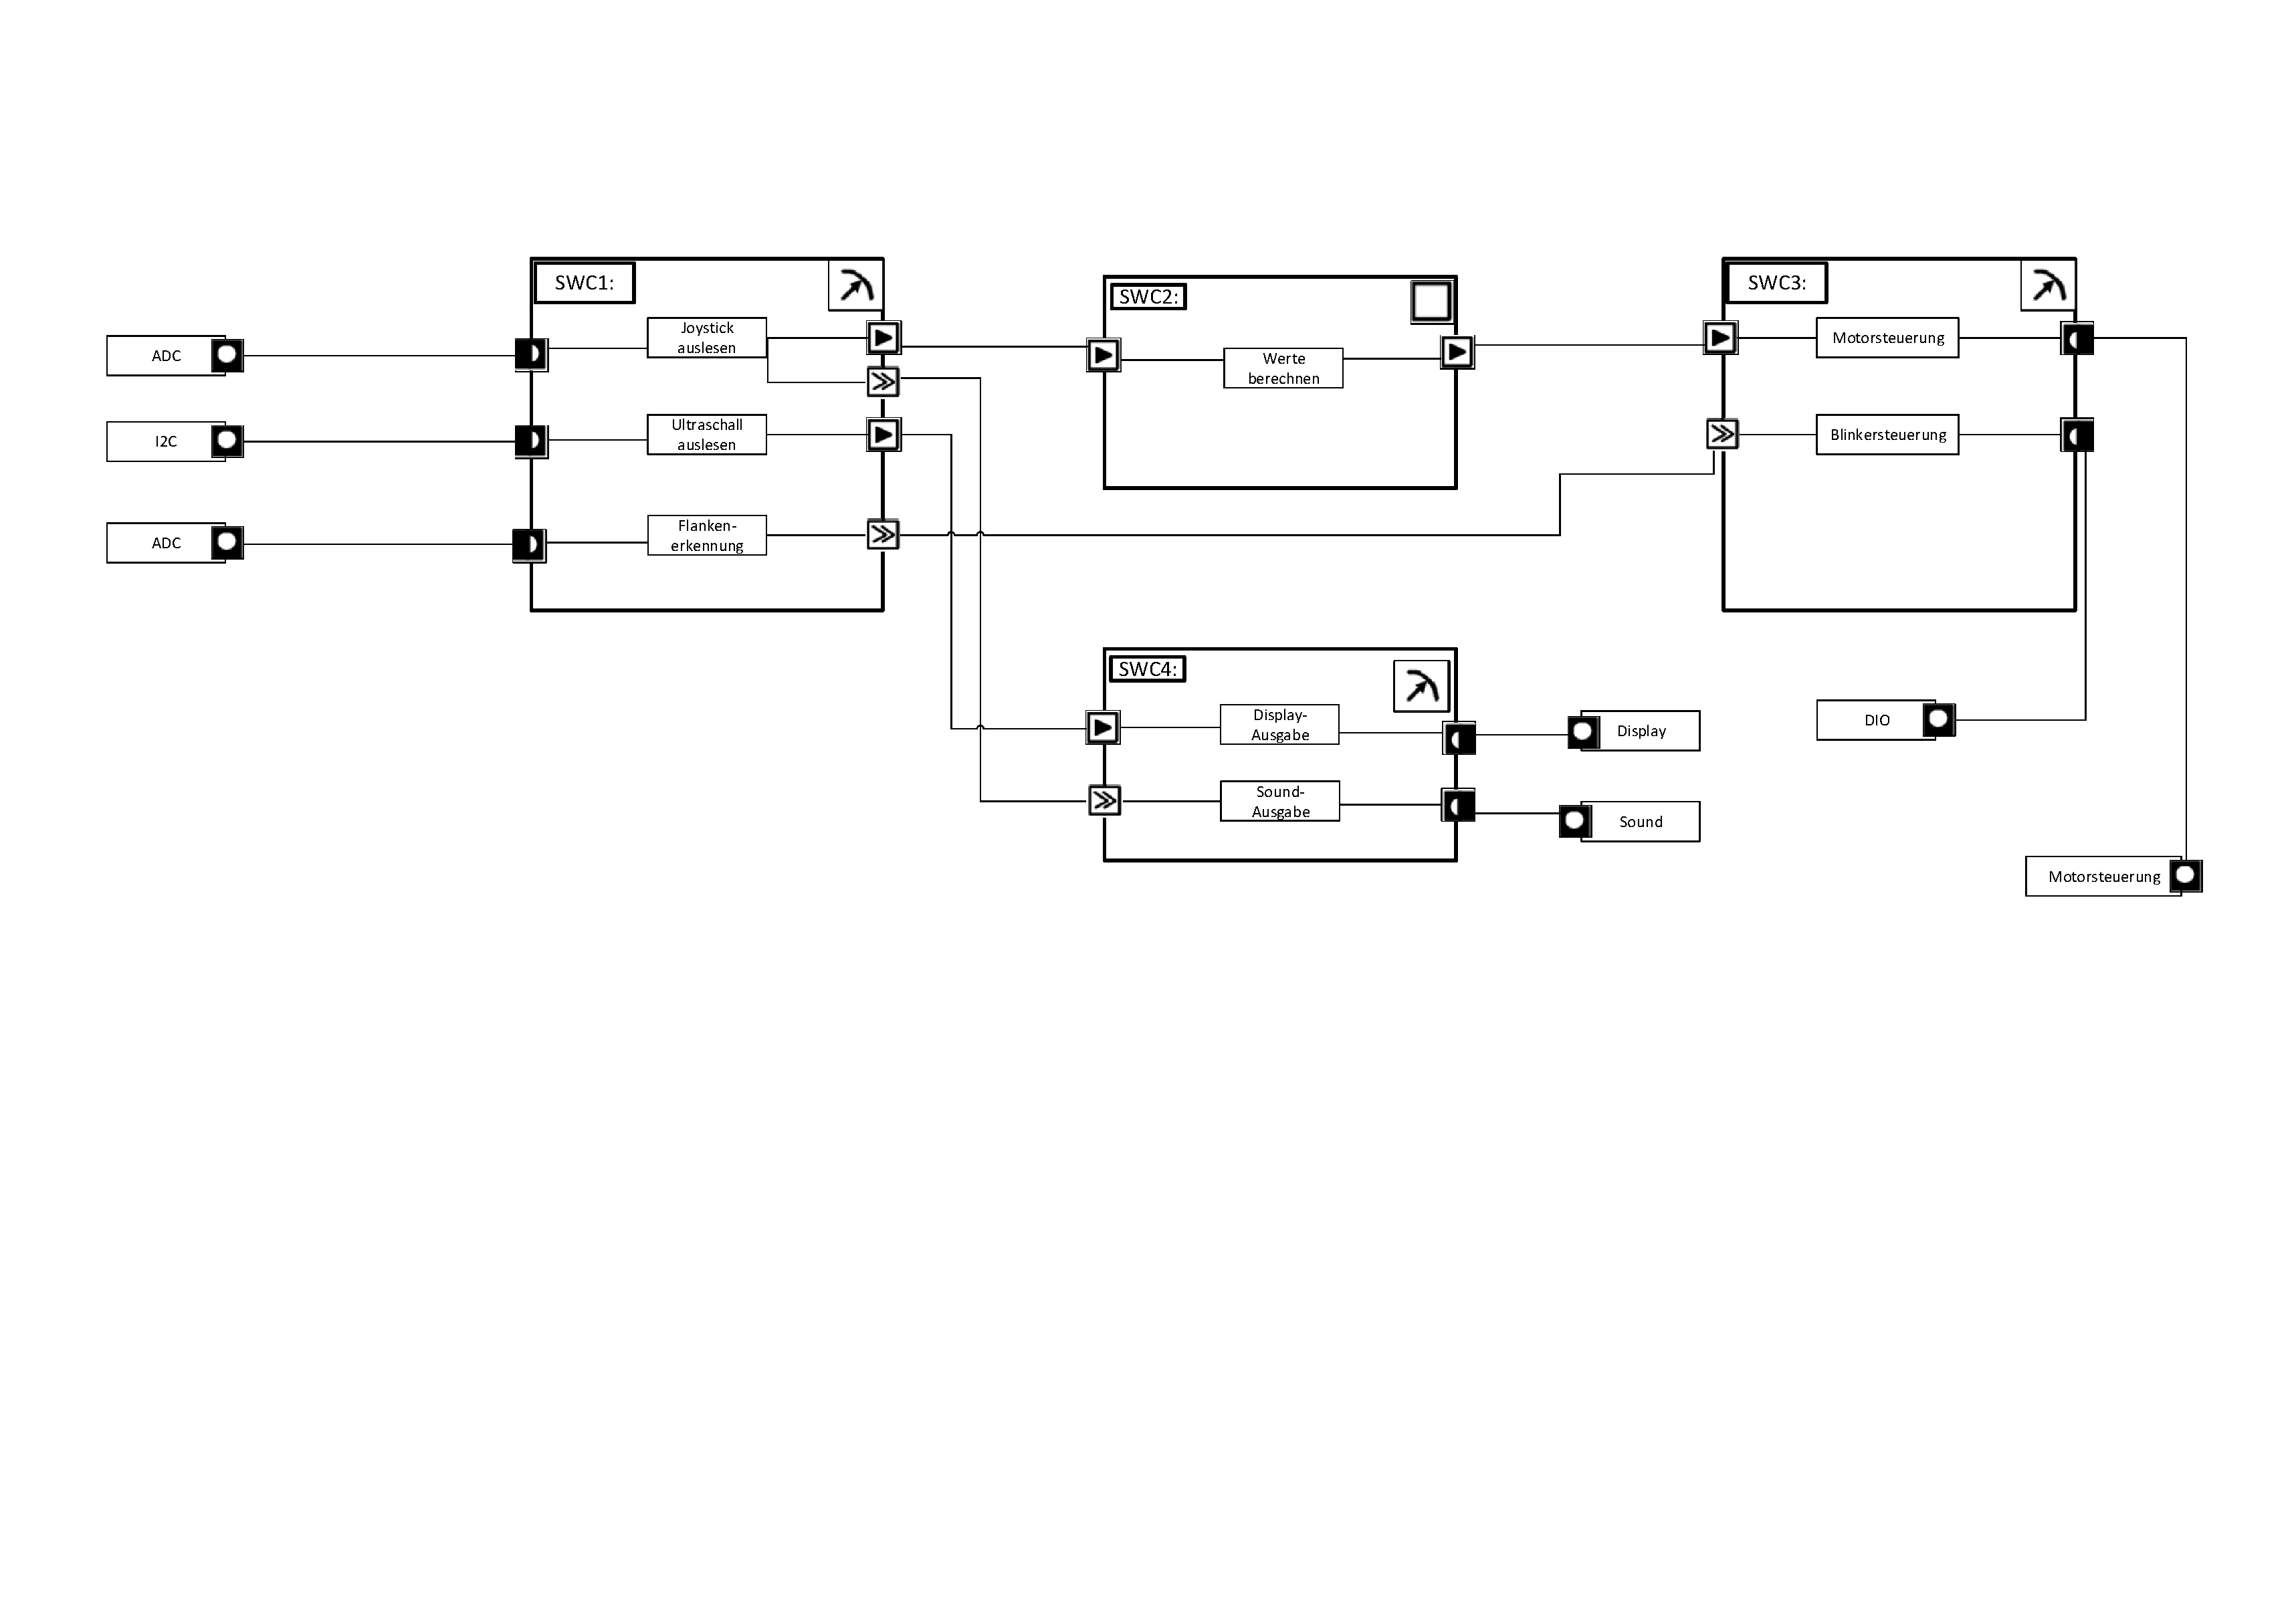
\includegraphics[scale=0.35,page=1]{Dokumente/ComponentDiagram.pdf}
\caption{Übersicht der Softwarekomponenten}
\label{pic:Softwarekompo}
\end{figure}
\end{landscape}
\newpage